\documentclass[11pt]{article}
\usepackage[margin=1in]{geometry}
\usepackage{amsmath,amssymb,amsthm,mathtools}
\usepackage{graphicx}
\usepackage{microtype}
\usepackage{enumitem}
\usepackage[hidelinks]{hyperref}

\newtheorem{theorem}{Theorem}
\newtheorem{corollary}[theorem]{Corollary}
\newtheorem{proposition}[theorem]{Proposition}
\newtheorem{lemma}[theorem]{Lemma}
\theoremstyle{remark}
\newtheorem{remark}[theorem]{Remark}

\newcommand{\N}{\mathbb N}
\newcommand{\Pp}{\mathbb P}
\newcommand{\Ee}{\mathbb E}
\newcommand{\Law}{\mathcal L}
\newcommand{\Bn}{\mathsf B}
\newcommand{\Gsample}{\mathbb G^{\mathrm R}}

\title{A sharp moment-theoretic bridge between\\
sampling and node-and-edge convergence}
\author{Candidate partial result for arXiv:1406.7846}
\date{17 August 2026}

\begin{document}
\maketitle

\begin{center}
\fbox{\parbox{0.92\textwidth}{\textbf{Status.}
Candidate substantial partial result, likely valid.  For genuine
probability-valued multigraphons, sampling convergence implies full
node-and-edge density convergence exactly when the one-edge bond moments
converge.  Conversely, density convergence implies sampling convergence when
the limiting one-edge moment sequence is Stieltjes-determinate.  In
particular, the notions are equivalent under one uniform exponential-moment
bound.  Counterexamples show that uniform integrability and moment
determinacy are the two genuine obstructions.}}
\end{center}

\section{Source question}

Kunszenti-Kov\'acs, Lov\'asz, and Szegedy study multigraph limits with
unbounded edge multiplicities in \cite{KLS}.  In Section~4.4 they recall that
homomorphism-density convergence and finite-sample convergence coincide for
bounded or compact decorations and then ask what happens for unbounded
multigraphs.  They isolate the unboundedness of the density tests and moment
indeterminacy as obstacles, give a counterexample in full generality, and
conclude that they expect settings where the notions coincide but do not
investigate them.

The question and its two stated obstructions appear on source PDF page~32:

\begin{center}

\includegraphics[width=\textwidth]{figures/open_problem_crop.png}
\end{center}

The explicit expected-settings sentence is on source PDF page~33:

\begin{center}
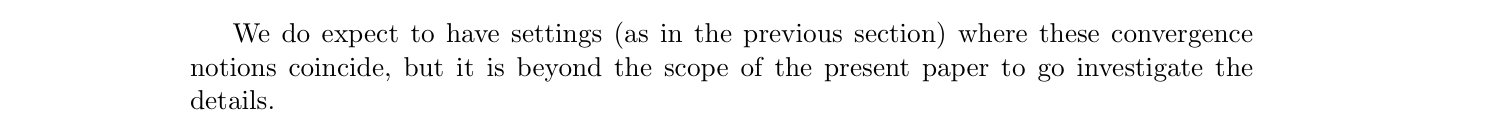
\includegraphics[width=\textwidth]{figures/open_problem_scope_crop.png}
\end{center}

The theorem below identifies the two obstacles exactly enough to give a broad
positive regime and two sharp failure examples.

\section{Framework and the mixed-moment identity}

A \emph{probability multigraphon} is a symmetric measurable kernel
\[
 W:[0,1]^2\longrightarrow \mathcal P(\N_0).
\]
For the random $k$-vertex sample $\Gsample(k,W)$, first choose independent
uniform latent variables $X_1,\ldots,X_k$.  Conditional on them, choose the
edge multiplicities $M_{ij}$ independently with law $W(X_i,X_j)$.

Let $F$ be a finite loopless multigraph on $[k]$.  Write $E_+(F)$ for the set
of unordered vertex-pairs having positive multiplicity and $r_e\geq1$ for the
multiplicity of $e\in E_+(F)$.  Then conditional independence gives the basic
identity
\begin{equation}\label{eq:mixed}
 t(F,W)=\Ee\prod_{e\in E_+(F)}M_e^{r_e}.
\end{equation}
Indeed, conditional on $X_1,\ldots,X_k$, both sides equal the product of the
$r_e$th moments of the corresponding edge laws.  If $\Bn_p$ denotes the
two-vertex multigraph with $p$ parallel edges, then
\begin{equation}\label{eq:bond}
 t(\Bn_p,W)=\Ee M_{12}^{p}.
\end{equation}
Thus node-and-edge densities are precisely the mixed polynomial moments of
the finite sampled edge vector.

Throughout, every $W_n$ is assumed to have finite bond moments of every
order.  Weak convergence of sample laws is ordinary weak convergence of
probability measures on the discrete Polish space
$\N_0^{\binom{k}{2}}$.

\section{Proof intuition}

There are two directions, and each source obstruction has one standard
probabilistic cure.

For sampling-to-density convergence, weak convergence already handles every
bounded test.  A density is an unbounded mixed monomial, so the missing
ingredient is uniform integrability.  Generalized H\"older reduces the
$L^2$ norm of any such mixed monomial to finitely many one-edge moments.
Consequently, once the bond moments converge, every density converges; no
regularity or cut-metric argument is needed.

For density-to-sampling convergence, the first bond moment makes each finite
family of sample laws tight.  All subsequential limits have the same mixed
moments, because higher bond moments again give uniform integrability.
Marginal Stieltjes determinacy then invokes the half-line version of
Petersen's theorem: determinate coordinate marginals make the whole joint law
determinate.  A uniform exponential moment supplies both uniform
integrability and Carleman's determinacy criterion, yielding a clean
two-way equivalence.  The original question remains broader for arbitrary
moment-indeterminate families and for quotient-valued graphons without a
chosen probability-kernel representative.

\section{The moment bridge}

\begin{lemma}[Mixed-monomial uniform integrability]\label{lem:UI}
Let $Z_n=(Z_{n,1},\ldots,Z_{n,q})$ be nonnegative random vectors.  Fix positive
integers $r_1,\ldots,r_q$.  If
\[
 \sup_n \Ee Z_{n,j}^{,2q r_j}<\infty
 \qquad(1\leq j\leq q),
\]
then $Y_n=\prod_{j=1}^q Z_{n,j}^{r_j}$ is uniformly integrable.
\end{lemma}

\begin{proof}
Generalized H\"older with all exponents equal to $q$ gives
\begin{equation}\label{eq:holder}
 \Ee Y_n^2
 =\Ee\prod_{j=1}^q Z_{n,j}^{,2r_j}
 \leq \prod_{j=1}^q
 \left(\Ee Z_{n,j}^{,2q r_j}\right)^{1/q}.
\end{equation}
The right side is uniformly bounded.  Hence $(Y_n)$ is bounded in $L^2$ and
is uniformly integrable.
\end{proof}

\begin{theorem}[Sampling/density moment bridge]\label{thm:bridge}
Let $(W_n)$ be probability multigraphons with all finite bond moments.

\begin{enumerate}[label=\textup{(\roman*)},leftmargin=2.2em]
\item\label{it:forward}
Suppose $\Law(\Gsample(k,W_n))$ converges weakly for every $k$.  Then
$(W_n)$ is node-and-edge density convergent if and only if
\[
 \lim_{n\to\infty}t(\Bn_p,W_n)
\]
exists and is finite for every $p\geq1$.

\item\label{it:reverse}
Suppose $t(F,W_n)$ converges for every finite loopless multigraph $F$, and put
\[
 m_p=\lim_{n\to\infty}t(\Bn_p,W_n),\qquad m_0=1.
\]
If $(m_p)_{p\geq0}$ is determinate for the Stieltjes moment problem on
$[0,\infty)$, then $\Law(\Gsample(k,W_n))$ converges weakly for every $k$.
\end{enumerate}
\end{theorem}

\begin{proof}
For \ref{it:forward}, necessity is immediate because each $\Bn_p$ is itself a
test multigraph.  Conversely, fix $F$ on $[k]$, enumerate its $q$ positive
edge-pairs as $e_1,\ldots,e_q$, and let their multiplicities be
$r_1,\ldots,r_q$.  The sampled edge vector converges in law by hypothesis.
For every $j$,
\[
 \Ee (M_{e_j}^{(n)})^{2qr_j}=t(\Bn_{2qr_j},W_n),
\]
which is uniformly bounded because it converges.  Lemma~\ref{lem:UI} makes
$\prod_j(M_{e_j}^{(n)})^{r_j}$ uniformly integrable.  Convergence in law plus
uniform integrability, followed by \eqref{eq:mixed}, proves convergence of
$t(F,W_n)$.

For \ref{it:reverse}, fix $k$ and put $d=\binom{k}{2}$.  Let $\nu_{n,k}$ be
the law of the full $d$-coordinate sampled edge vector.  Exchangeability and
Markov's inequality give, for $R>0$,
\begin{equation}\label{eq:tight}
 \nu_{n,k}\!\left\{\max_e M_e>R\right\}
 \leq \sum_e\frac{\Ee M_e}{R}
 =\frac{d\,t(\Bn_1,W_n)}{R}.
\end{equation}
The last numerator is bounded, so $(\nu_{n,k})_n$ is tight.

Consider any weakly convergent subsequence, with limit $\nu$.  For a
multi-index $a=(a_e)_{e=1}^d\in\N_0^d$, apply Lemma~\ref{lem:UI} to the
coordinates with $a_e>0$.  The required higher marginal moments are bounded
bond densities.  Therefore the monomial $x^a$ is uniformly integrable and
\begin{equation}\label{eq:mompass}
 \int x^a\,d\nu(x)
 =\lim_n \Ee\prod_e(M_e^{(n)})^{a_e}.
\end{equation}
The right side is the limiting density of the multigraph on $[k]$ having
multiplicity $a_e$ on pair $e$, so it is independent of the chosen
subsequence.  In particular, every coordinate marginal of $\nu$ has moment
sequence $(m_p)$.

The half-line extension of Petersen's marginal-determinacy theorem
\cite{DLY,Petersen} says that a measure on $[0,\infty)^d$ is determined by its
mixed moments whenever each coordinate marginal is Stieltjes-determinate.
Thus the common mixed moments in \eqref{eq:mompass} determine $\nu$ uniquely.
Every weak cluster point of the tight sequence $(\nu_{n,k})$ is consequently
the same, so the full sequence converges.  Since $k$ was arbitrary, the claim
follows.
\end{proof}

\begin{remark}[A moment-bounded forward criterion]\label{rem:bounded}
In Theorem~\ref{thm:bridge}\ref{it:forward}, it is enough to assume
\[
 \sup_n t(\Bn_p,W_n)<\infty\qquad\text{for every }p\geq1.
\]
Indeed, weak convergence of the two-vertex samples, together with the bounded
moment of order $p+1$, makes the $p$th powers uniformly integrable and hence
forces convergence of the $p$th bond moments.  This recovers the precise
uniform-integrability mechanism suggested by the moment-bounded part of the
source theory.
\end{remark}

\section{A concrete equivalence regime}

\begin{corollary}[Uniform exponential tails]\label{cor:exp}
Suppose there are constants $\alpha>0$ and $C<\infty$ such that
\begin{equation}\label{eq:exp}
 \sup_n\int_{[0,1]^2}
 \sum_{m=0}^{\infty}e^{\alpha m}
 W_n(x,y)\{m\}\,dx\,dy\leq C.
\end{equation}
Then the following are equivalent:
\begin{enumerate}[label=\textup{(\alph*)},leftmargin=2em]
\item $t(F,W_n)$ converges for every finite loopless multigraph $F$;
\item $\Law(\Gsample(k,W_n))$ converges weakly for every $k$.
\end{enumerate}
\end{corollary}

\begin{proof}
Let $M_n$ have the integrated one-edge law of $W_n$.  Condition
\eqref{eq:exp} says $\sup_n\Ee e^{\alpha M_n}\leq C$.

If the sample laws converge, then for every $p$, the variables $M_n^p$ are
uniformly integrable (for example, $x^p$ is dominated by a constant multiple
of $e^{\alpha x/2}$, whose squares have uniformly bounded expectation).
Thus their moments converge, and
Theorem~\ref{thm:bridge}\ref{it:forward} gives density convergence.

Conversely, suppose the densities converge.  Since
$x^p\leq p!\alpha^{-p}e^{\alpha x}$ for $x\geq0$, their limiting bond moments
satisfy
\begin{equation}\label{eq:factorial}
 m_p\leq C p!\alpha^{-p}.
\end{equation}
Consequently
\[
 \sum_{p=1}^{\infty}m_{2p}^{-1/(2p)}=\infty,
\]
because $((2p)!)^{1/(2p)}\leq 2p$.  Carleman's criterion makes the marginal
moment sequence Hamburger-determinate, hence Stieltjes-determinate.  Apply
Theorem~\ref{thm:bridge}\ref{it:reverse}.
\end{proof}

\begin{remark}[Joint exponential control]
For a $k$-vertex sample with $d=\binom{k}{2}$ edge coordinates, generalized
H\"older also gives
\[
 \Ee\exp\!\left(\frac{\alpha}{d}\sum_e M_e\right)
 \leq\prod_e\left(\Ee e^{\alpha M_e}\right)^{1/d}
 \leq C.
\]
Thus the one-edge hypothesis automatically controls every finite sample
jointly; no independence assumption is needed for this estimate.
\end{remark}

\section{Why the hypotheses cannot simply be omitted}

\begin{proposition}[Two sharp failure mechanisms]\label{prop:sharp}
Neither direction holds without its corresponding moment mechanism.

\begin{enumerate}[label=\textup{(\alph*)},leftmargin=2em]
\item There are probability multigraphons whose samples converge for every
$k$ but whose node-and-edge densities do not converge.
\item There are probability multigraphons whose node-and-edge densities all
converge but whose two-vertex sample laws do not converge.
\end{enumerate}
\end{proposition}

\begin{proof}
For (a), let $W_n$ be the constant kernel with edge law
\[
 \mu_n=\left(1-\frac1n\right)\delta_0+\frac1n\delta_n.
\]
In a fixed $k$-vertex sample, the probability that any of the
$d=\binom{k}{2}$ edges is nonzero is at most $d/n$.  Hence the sample law
converges in total variation to the zero multigraph.  On the other hand,
\[
 t(\Bn_2,W_n)=\int m^2\,d\mu_n(m)=n\longrightarrow\infty.
\]

For (b), use the distinct probability laws $\sigma$ and $\tau$ on $\N_0$
with all finite moments equal whose existence is recorded explicitly in
Examples~4.9 and~4.11 of \cite{KLS}.  Let $W_{2n}$ be the constant kernel
$\sigma$ and $W_{2n+1}$ the constant kernel $\tau$.  For every $F$,
\[
 t(F,W_n)=\prod_{e\in E_+(F)}
 \int m^{r_e}\,d\sigma(m)
 =\prod_{e\in E_+(F)}
 \int m^{r_e}\,d\tau(m),
\]
so the density is independent of $n$.  Yet the two-vertex sample law
alternates between the distinct laws $\sigma$ and $\tau$.
\end{proof}

The second example shows that determinacy is the sharp obstruction to a
\emph{general} moments-to-law implication.  It does not say that determinacy
is necessary for a particular already-convergent sequence.

\section{Verification, limitations, and novelty status}

The proof has four check points.  First, \eqref{eq:mixed} is conditional
independence applied to a single sampled multiplicity per vertex-pair.
Second, \eqref{eq:holder} uses only marginal moments and therefore does not
assume unconditional independence of the sampled edges.  Third,
\eqref{eq:tight} gives finite-dimensional tightness before subsequences are
taken.  Fourth, all mixed moments pass to a subsequential limit by the same
$L^2$ uniform-integrability estimate, after which the cited half-line
marginal-determinacy theorem applies.  The two counterexamples have also been
checked directly.

This packet applies to genuine $\mathcal P(\N_0)$-valued kernels and to finite
multigraphs through their step kernels.  It does not solve the measurable
selection issue for the source's quotient-valued moment graphons.  Nor does it
give a non-tautological necessary-and-sufficient criterion for every
individual moment-indeterminate density-convergent sequence.  For these
reasons the result is classified as a substantial partial answer rather than
a full solution of the source's broad-ended question.

A bounded novelty search on 17 August 2026 used the exact source title and
arXiv id, its citation neighborhood, and the phrases ``node-and-edge sample
convergence'', ``multigraphon sampling moment determinate'', ``Petersen
theorem graphon'', and ``Carleman sample convergence graphon''.  The closest
results found were Kunszenti-Kov\'acs's Carleman-based uniqueness theorem for
Banach-valued graphons \cite{KK} and the probability-graphon equivalence of
sampling, cut convergence, and homomorphism tests with bounded continuous
edge decorations due to Abraham--Delmas--Weibel \cite{ADW}.  The former is a
graphon weak-isomorphism theorem; the latter uses bounded $C_b$ tests, not the
unbounded polynomial tests defining node-and-edge multigraph densities.  No
exact occurrence of Theorem~\ref{thm:bridge} or Corollary~\ref{cor:exp} was
found.  Novelty confidence is moderate, not definitive.

\paragraph{Human-review recommendation.}
Check the identification \eqref{eq:mixed}, the exponents $2qr_j$ in
\eqref{eq:holder}, and the support hypotheses in the half-line Petersen
theorem.  If those pass, retain this as a substantial partial theorem giving
an exact forward criterion, a determinate reverse theorem, and a concrete
two-way equivalence regime.

\begin{thebibliography}{9}
\bibitem{KLS}
D. Kunszenti-Kov\'acs, L. Lov\'asz, and B. Szegedy,
\emph{Multigraph limits, unbounded kernels, and Banach space decorated
graphs}, J. Funct. Anal. \textbf{282} (2022), Article 109284;
arXiv:1406.7846, doi:10.1016/j.jfa.2021.109284.

\bibitem{Petersen}
L. C. Petersen,
\emph{On the relation between the multidimensional moment problem and the
one-dimensional moment problem}, Math. Scand. \textbf{51} (1982), 361--366;
doi:10.7146/math.scand.a-11986.

\bibitem{DLY}
A. Dvure\v{c}enskij, P. Lahti, and K. Ylinen,
\emph{The uniqueness question in the multidimensional moment problem with
applications to phase space observables}, Rep. Math. Phys. \textbf{50}
(2002), 55--68; arXiv:quant-ph/0108059,
doi:10.1016/S0034-4877(02)80044-1.

\bibitem{KK}
D. Kunszenti-Kov\'acs,
\emph{Uniqueness of Banach space valued graphons}, J. Math. Anal. Appl.
\textbf{474} (2019), 413--440; arXiv:1504.01263,
doi:10.1016/j.jmaa.2019.01.052.

\bibitem{ADW}
R. Abraham, J.-F. Delmas, and J. Weibel,
\emph{Probability-graphons: Limits of large dense weighted graphs},
Innov. Graph Theory \textbf{2} (2025), 25--117; arXiv:2312.15935,
doi:10.5802/igt.7.
\end{thebibliography}

\end{document}
